\section{parte 04 – Desarrollo} 

\begin{enumerate}[1.]
	\item PROCEDIMIENTOS PARA LA CREACIÓN DE COPIAS:


	\item BACKUPS  DESDE  ENTERPRISE  MANAGER:
	

	\item RECUPERACIÓN  DESDE  ENTERPRISE  MANAGER
	\\\\Para realizar una recuperación desde EM, iremos a “Disponibilidad” y seleccionamos Realizar Recuperación
	\begin{center}
	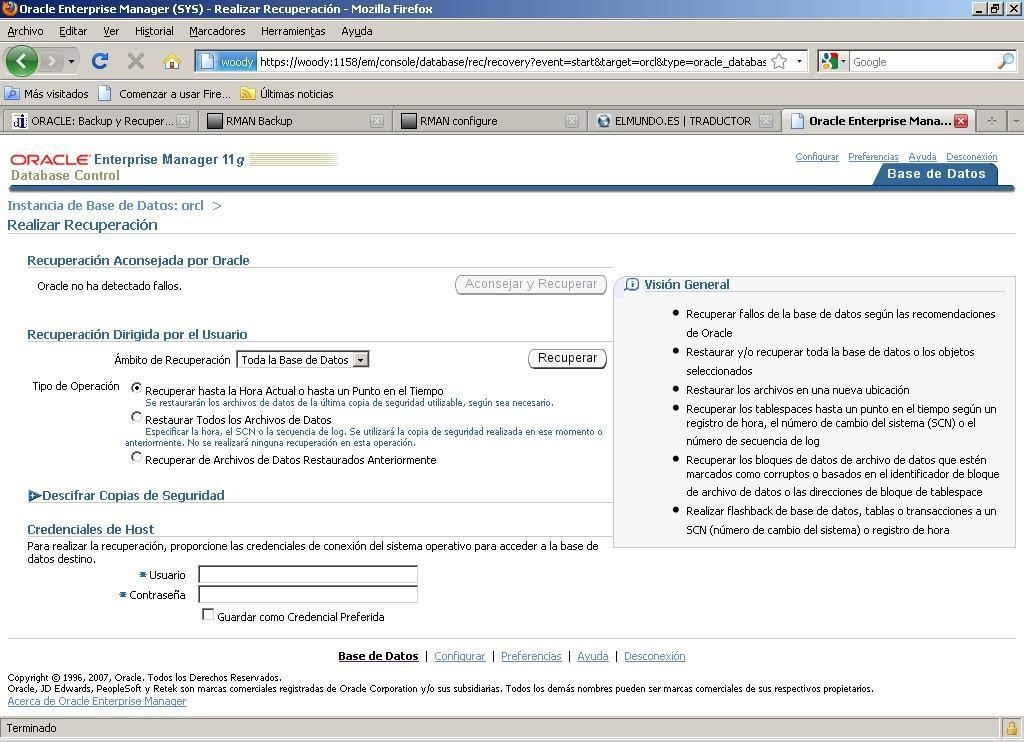
\includegraphics[width=15cm]{./Imagenes/recu_1}  
	\end{center}	
	En ámbitos de recuperación podemos seleccionar toda o parte de la base de datos para recuperar.
Para  el  ejemplo  hemos  borrado  el  datafile  USERS01.DBF(OFFLINE)  después  de realizar el backup y ahora vamos a intentar recuperarlo. Para ello usaremos la copia que acabamos de realizar. Iniciamos oracle en modo mount y arrancamos EM. Al no poder iniciar nos encontramos con esto una vez logueados.
	\begin{center}
	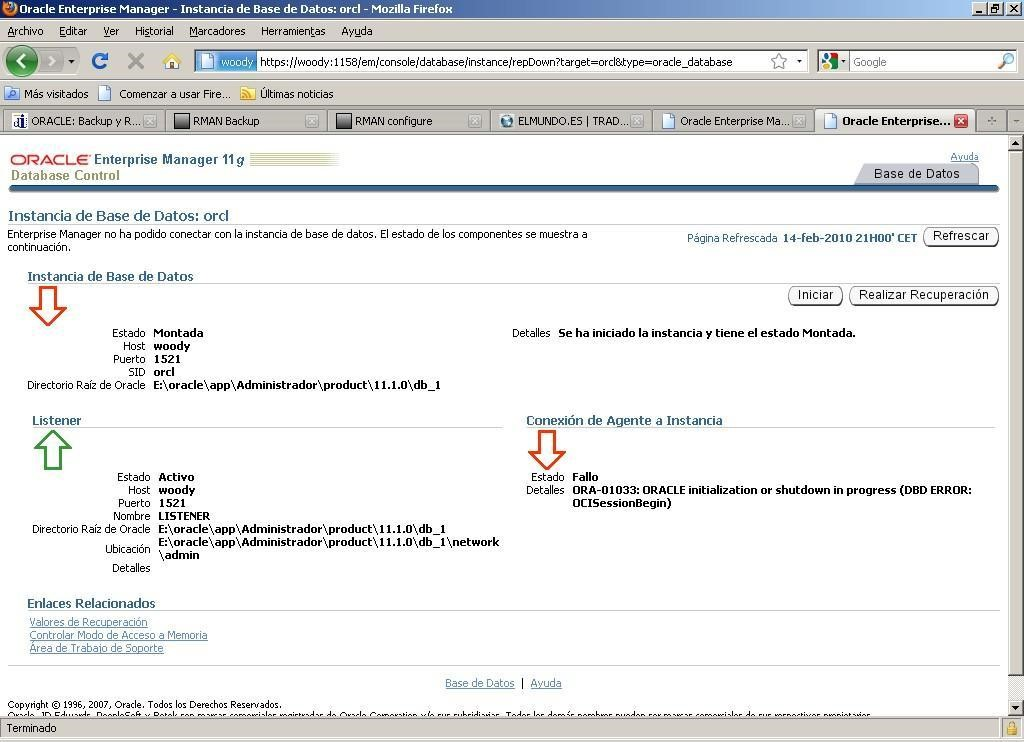
\includegraphics[width=15cm]{./Imagenes/recu_2}  
	\end{center}
	Pinchamos en Realizar Recuperación. Introducimos los credenciales de host. Continuar Nos conectamos como sysdba.
	\begin{center}
	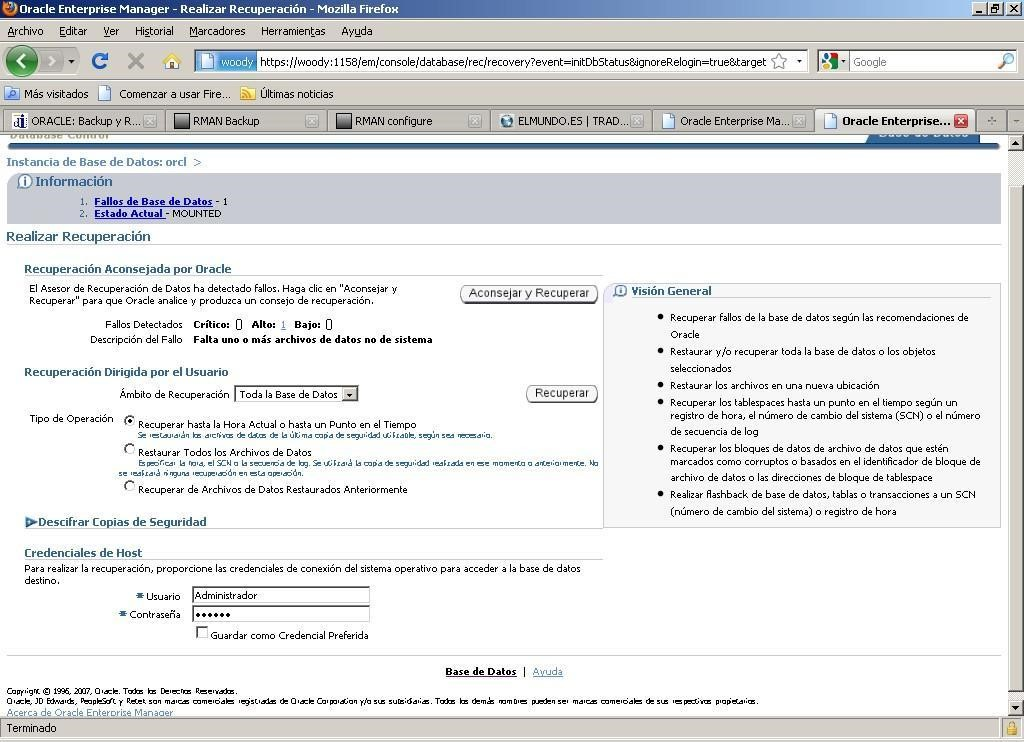
\includegraphics[width=15cm]{./Imagenes/recu_3}  
	\end{center}
	En el ámbito de recuperación elegimos Archivos de Datos y en el tipo de operación restaurar hasta hora actual. Pinchamos en recuperar.
	\begin{center}
	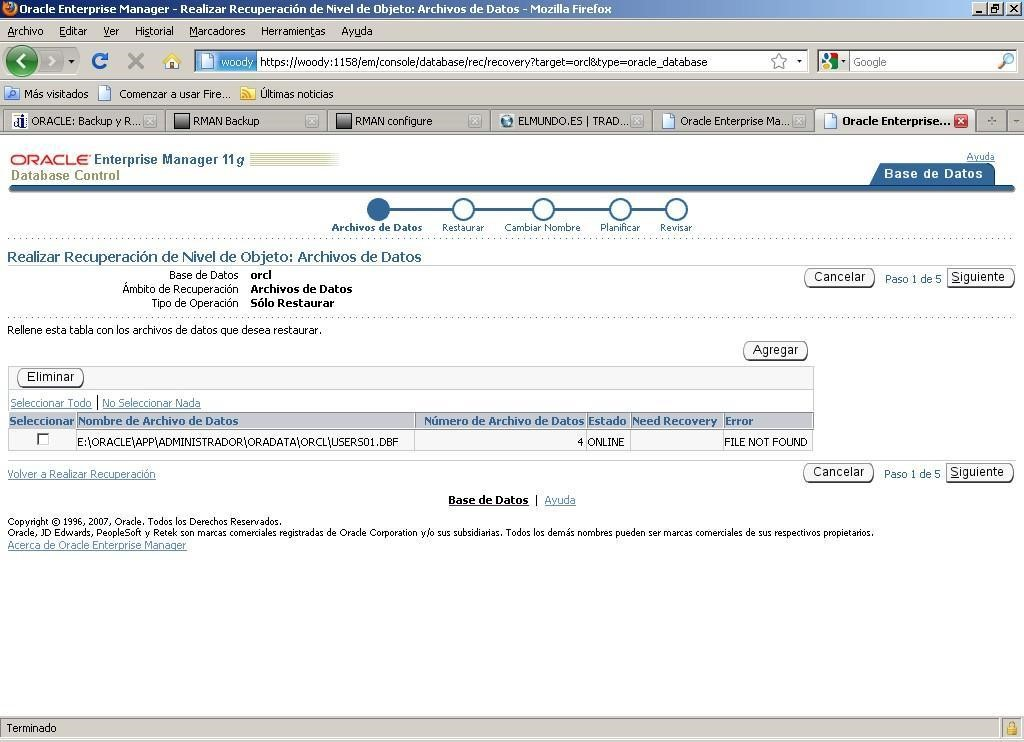
\includegraphics[width=15cm]{./Imagenes/recu_4}  
	\end{center}	
	Vemos  como  EM  localiza  la  ruta  en  conflicto  y  te  la  presenta  para  seleccionarla. Siguiente.
	\begin{center}
	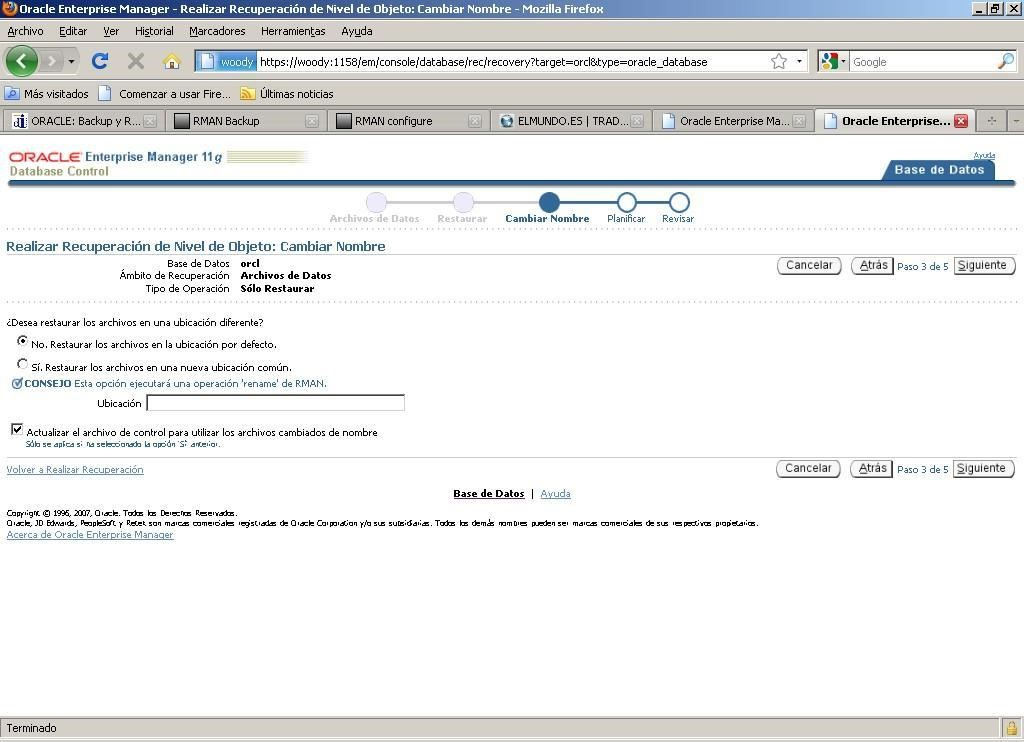
\includegraphics[width=15cm]{./Imagenes/recu_5}  
	\end{center}	
	También podemos definir el destino de la restauración. Para el ejemplo nos interesa que se ubiquen en el mismo directorio.
	\begin{center}
	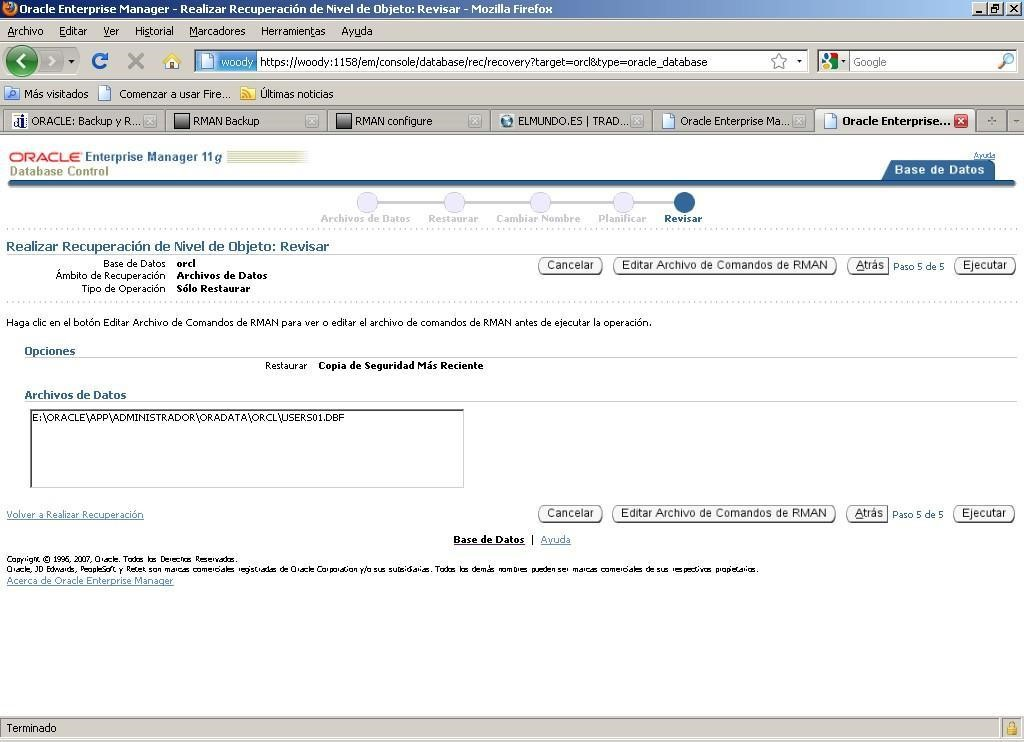
\includegraphics[width=15cm]{./Imagenes/recu_6}  
	\end{center}	
	Podemos revisar los parámetros RMAN para ver y comprender las acciones realizadas por debajo de EM. Una vez toda revisado procedemos a ejecutar.
	\\Esto lo que hará será tomar del backup el fichero y llevarlo al destino aplicando los cambios  hasta  el  momento  de  la  pérdida  permitiendo  así  el  inicio  normal  de  la  BD  con tablespace online.
	\\Una vez finalizado podemos pinchar en Abrir Base de Datos y esta se reiniciará y se abría automáticamente después de ver insertado nuestros credenciales.
	


\end{enumerate} 
